\documentclass[border=10pt]{standalone}
\usepackage{tikz}
\usetikzlibrary{arrows.meta,calc}

\begin{document}
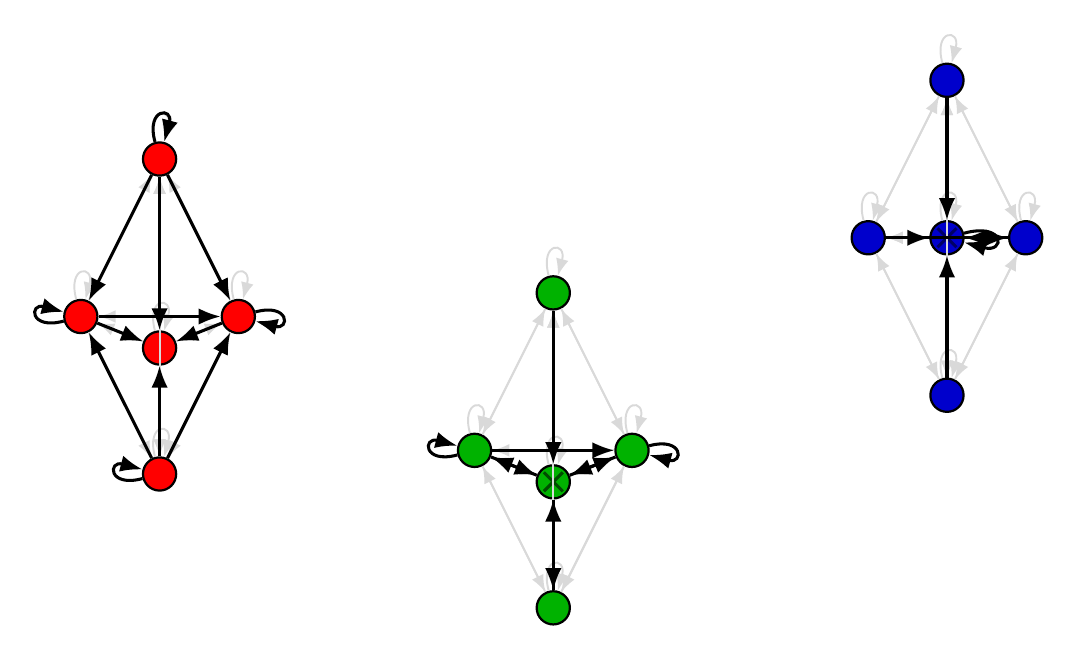
\begin{tikzpicture}[
  >=Latex,
  node distance=2cm,
  every node/.style={circle,draw=black,thick,minimum size=12pt,inner sep=0pt},
  bgedge/.style={gray!30, line width=0.7pt, ->},
  fgedge/.style={black, line width=1.1pt, ->},
  loopbg/.style={gray!30, line width=0.7pt, ->},
  loopfg/.style={black, line width=1.1pt, ->}
]

% Helper macro: draw complete digraph with loops for given set of nodes
\newcommand{\completeDG}[1]{%
  % directed edges between distinct nodes
  \foreach \i in {1,...,5}{%
    \foreach \j in {1,...,5}{%
      \ifnum\i=\j\relax\else
        \draw[bgedge] (#1\i) -- (#1\j);
      \fi
    }%
  }%
  % loops
  \foreach \i in {1,...,5}{%
    \draw[loopbg] (#1\i) edge[loop above, looseness=10] (#1\i);
  }%
}

%%%%%%%%%%%%%%%%%%%%
% 1) RED GRAPH LEFT
%%%%%%%%%%%%%%%%%%%%
\begin{scope}[shift={(-5,0)}]
  % Node placement: 1=top,2=left,3=right,4=bottom,5=center
  \node[fill=red] (R1) at (0,2) {};
  \node[fill=red] (R2) at (-1,0) {};
  \node[fill=red] (R3) at (1,0) {};
  \node[fill=red] (R4) at (0,-2) {};
  \node[fill=red] (R5) at (0,-0.4) {};

  % background complete digraph
  \completeDG{R}

  % foreground self loops on specific nodes
  \draw[loopfg] (R1) edge[loop above, looseness=10] (R1);
  \draw[loopfg] (R2) edge[loop left,  looseness=10] (R2);
  \draw[loopfg] (R3) edge[loop right, looseness=10] (R3);
  \draw[loopfg] (R4) edge[loop left,  looseness=10] (R4);

  % foreground emphasized edges
  \draw[fgedge] (R1) -- (R5);      % top to center
  \draw[fgedge] (R1) -- (R2);      % top to left
  \draw[fgedge] (R1) -- (R3);      % top to right
  \draw[fgedge] (R2) -- (R5);
  \draw[fgedge] (R3) -- (R5);
  \draw[fgedge] (R2) -- (R3);
  \draw[fgedge] (R4) -- (R2);
  \draw[fgedge] (R4) -- (R3);
  \draw[fgedge] (R4) -- (R5);
\end{scope}

%%%%%%%%%%%%%%%%%%%%
% 2) GREEN GRAPH CENTER
%%%%%%%%%%%%%%%%%%%%
\begin{scope}[shift={(0,-1.7)}]
  % Nodes
  \node[fill=green!70!black] (G1) at (0,2) {};
  \node[fill=green!70!black] (G2) at (-1,0) {};
  \node[fill=green!70!black] (G3) at (1,0) {};
  \node[fill=green!70!black] (G4) at (0,-2) {};
  \node[fill=green!70!black] (G5) at (0,-0.4) {};

  % put X on center node
  \draw[green!30!black, line width=1.1pt] ($(G5.center)+(-0.12,-0.12)$) --
                                       ($(G5.center)+(0.12,0.12)$);
  \draw[green!30!black, line width=1.1pt] ($(G5.center)+(-0.12,0.12)$) --
                                       ($(G5.center)+(0.12,-0.12)$);

  % background
  \completeDG{G}

  % foreground loops only on left/right mid nodes
  \draw[loopfg] (G2) edge[loop left,  looseness=10] (G2);
  \draw[loopfg] (G3) edge[loop right, looseness=10] (G3);

  % foreground edges
  \draw[fgedge] (G1) -- (G5);
  \draw[fgedge] (G2) -- (G5);
  \draw[fgedge] (G3) -- (G5);
  \draw[fgedge] (G4) -- (G5);
  \draw[fgedge] (G5) -- (G4);
  \draw[fgedge] (G5) -- (G2);
  \draw[fgedge] (G5) -- (G3);
  \draw[fgedge] (G2) -- (G3);
\end{scope}

%%%%%%%%%%%%%%%%%%%%
% 3) BLUE GRAPH RIGHT
%%%%%%%%%%%%%%%%%%%%
\begin{scope}[shift={(5,1)}]
  % Nodes (compact)
  \node[fill=blue!80!black] (B1) at (0,2) {};
  \node[fill=blue!80!black] (B2) at (-1,0) {};
  \node[fill=blue!80!black] (B3) at (1,0) {};
  \node[fill=blue!80!black] (B4) at (0,-2) {};
  \node[fill=blue!80!black] (B5) at (0,0) {};

  % X on center
  \draw[blue!40!black, line width=1.1pt] ($(B5.center)+(-0.12,-0.12)$) --
                                       ($(B5.center)+(0.12,0.12)$);
  \draw[blue!40!black, line width=1.1pt] ($(B5.center)+(-0.12,0.12)$) --
                                       ($(B5.center)+(0.12,-0.12)$);

  % background
  \completeDG{B}

  % foreground loop only on center
  \draw[loopfg] (B5) edge[loop right, looseness=12] (B5);

  % foreground edges
  \draw[fgedge] (B1) -- (B5);
  \draw[fgedge] (B2) -- (B5);
  \draw[fgedge] (B3) -- (B5);
  \draw[fgedge] (B4) -- (B5);
  \draw[fgedge] (B2) -- (B3);  % horizontal
\end{scope}

\end{tikzpicture}
\end{document}